\documentclass[12pt]{report}
\usepackage[a4paper]{geometry}
\usepackage[myheadings]{fullpage}
\usepackage{fancyhdr}
\usepackage{lastpage}
\usepackage{graphicx, wrapfig, subcaption, setspace, booktabs}
\usepackage[T1]{fontenc}
\usepackage[font=small, labelfont=bf]{caption}
\usepackage{fourier}
\usepackage[protrusion=true, expansion=true]{microtype}
\usepackage[french]{babel}
\usepackage{sectsty}
\usepackage{url, lipsum}
\usepackage{tgbonum}
\usepackage{hyperref}
\usepackage{xcolor}
\usepackage{amssymb}
\usepackage{tikz}
\usepackage[utf8]{inputenc}
\usepackage{siunitx}
\usetikzlibrary{babel}
\usepackage[european, straightvoltages, RPvoltages, cuteinductors]{circuitikz}
\usepackage{pgfplots}
\usepackage{amsmath}
\usepackage{float}
\usepackage{bodegraph}
\graphicspath{ {./images/} }

\newcommand{\HRule}[1]{\rule{\linewidth}{#1}}
\onehalfspacing
\setcounter{tocdepth}{5}
\setcounter{secnumdepth}{5}

\renewcommand{\thesection}{\arabic{section}}
\renewcommand{\thesubsection}{\arabic{section}.\arabic{subsection}}

\begin{document}
{\fontfamily{ptm}\selectfont
\title{ \normalsize \textsc{}
		\\ [2.0cm]
		\HRule{0.5pt} \\
		\LARGE \textbf{\uppercase{RAPPORT ELECTRONIQUE VI}\\
        \textbf{Les filtres analogiques}
		\HRule{2pt} \\ [0.5cm]
		\normalsize \today \vspace*{5\baselineskip}}
		}

\date{}

\author{
		Nicolas Oscar - Mohamed Ali Irshad\\ 
		JUNIA ISEN Lille \\
		T1 CIR 1
}

\maketitle
\tableofcontents

\newpage
\section{Introduction \& Matériel Utilisé}
Le but de ce T.P. était d’étudier le fonctionnement d’une diode. Ce composant peut être utilisé dans le redressement de tensions alternatives et la commutation d’alimentation.
\\

Voic la liste du matériel que nous avons utilisé pour ce T.P. :

— 1 alimentation double \\
— 1 générateur basse fréquence (GBF)\\
— 1 oscilloscope + 2 sondes\\
— 1 potentiomètre\\
— 1 diode 1N4148\\
— Résistances et condensateurs divers

\newpage
\section{La diode}
\begin{figure}[H]
    \begin{center}
        \includegraphics*[scale=0.5]{images/1.png}
        \caption{\label{figure 1} Schéma d'un montage avec une diode, une résistance $R=270 \Omega$ et un GBF.}
    \end{center}
\end{figure}

Nous avons réalisé le montage précédent et avons ensuite mesuré la tension aux bornes de la diode, de la résistance et avons estimer en conséquence le courant du circuit en variant la tension d'entrée. Nous avons obtenu les résultats suivants :

\begin{table}[H]
    \centering
    \begin{tabular}{|c|c|c|c|c|c|c|c|c|c|c|c|c|}
        \hline
        $E$ (V) & -5 & -4 & -3 & -2 & -1 & 0 & 1 & 2 & 3 & 4 & 5\\
        \hline
        $V_D$ (V) & -5 & -4 & -3 & -2 & -1 & 0 & 0.63 & 0.69 & 0.72 & 0.74 & 0.77\\
        \hline
        $V_R$ (V)& 0 & 0 & 0 & 0 & 0 & 0 & 0.37 & 1.34 & 2.22 & 3.22 & 4.2\\
        \hline
        $I$ (mA) & 0 & 0 & 0 & 0 & 0 & 0 & 1.3 & 4.6 & 8.13 & 11.9 & 15.49\\
        \hline
    \end{tabular}
    \caption{\label{table 1} Tableau correspondant aux mesures de la figure \ref{figure 1}.}
\end{table}

\newpage
Voici ensuite la courbe représentant l'intensité du courant I en fonction de la tension $V_D$ : 

\begin{figure}[H]
    \begin{center}
    \begin{tikzpicture}
        \begin{axis}[
            xlabel={$V_D$},
            ylabel={$I$},
            xmin=-2,
            xmax=2,
            ymin=0,
            ymax=15,
            grid=both,
            grid style={line width=0.2pt, draw=gray!50},
            width=0.8\textwidth,
            height=0.6\textwidth,
            legend pos=north west,
            legend cell align={left},
            ytick distance=1, % Set the y-axis tick distance to 1
        ]
        
        % Plot the curv
        \addplot[blue, mark=*] coordinates {
            (-5, 0)
            (-4, 0)
            (-3, 0)
            (-2, 0)
            (-1, 0)
            (0, 0)
            (0.63, 1.3)
            (0.69, 4.6)
            (0.72, 8.13)
            (0.74, 11.9)
            (0.77, 15.49)
        };
        \addlegendentry{$I$}
        
        \end{axis}
    \end{tikzpicture}
    \caption{\label{graph 1} Courbe représentant l'intensité du courant I en fonction de la tension $V_D$.}
    \end{center}
\end{figure}

Nous pouvons distinguer deux états distincts qui sont : 

- Si la tension est négative, alors le courant est nul donc la diode est dite \underline{"bloquante"}

- Si la tension est positive, alors le courant est non nul donc la diode est dite \underline{"passante"}\\


La résistance dans ce circuit permet de simuler la résistance de la diode lorsque la tension est négative et que la diode soit "bloquante".

\newpage
\section{Pont de Wheatstone}
\underline{$\star$ Rappel :} 
- Une diode peut être modélisé de la manière suivante : 
\begin{figure}[H]
    \begin{center}
        \includegraphics*[scale=0.5]{images/2.png}
        \caption{\label{figure 2} Modélisation d'une diode.}
    \end{center}
\end{figure}
- Sur les ponts de Wheatstone :

$U_{AB} = 0V$ si $(R_1+R_2+xR_p)(R_4+R_D)=R_3R_5$

\begin{figure}[H]
    \begin{center}
        \includegraphics*[scale=0.5]{images/3.png}
        \caption{\label{figure 3} Schéma d'un montage avec $E_2=0V$, $R_1 = 100\Omega$,$R_2=820\Omega$,$R_3=150\Omega$,$R_4=47\Omega$ et $R_5=470\Omega$.}
    \end{center}
\end{figure}

Dans le cas d’une diode idéale, $R_D$ et $V_{th}$ sont nulles, mais cela n’est pas le cas pour un composant réel.
Le but de cet exercice était de déterminer les valeurs $R_D$ et $V_{th}$ des diodes disponibles en salle de TP.
\\

Nous avons reproduis le montage de la figure \ref{figure 3}, avons réglé le potentiomètre pour obtenir une tension de $U_{AB}=0V$ et avons ensuite, sans dérégler le potentiomètre, placé la diode et réglé le générateur $E_1 = 7V$ et $ E_2 = 0.69 $ pour avoir une tension $U_C = 0V$. 
\\

Le but d'une tel manipulation est de déterminer la valeur de la résistance du potentiomètre sans la
connaître par équilibrage des deux branches du circuit, En effet lorsque $U > V_{th}$ la diode se comporte
comme un générateur. On règle donc le générateur $E_2$ de manière à ce qu’il compense la tension $V_{th}$
afin de calculer $R_D$. Voici un schéma l'expliquant : 
\\

Ensuite, et ce sans déréglé $V_2$, nous avons réglé la valeur $E_1 = 10V$ et réglé de nouveau le potentiomètre pour obtenir une tension $ U_{AB}=0V$ :

\[(R_1+R_2+xR_p)(R_4+R_D)=R_3R_5\]
\[\leftrightarrow R_4+R_D = \frac{R_3R_5}{R_1+R_2+xR_p}\]
\[\leftrightarrow R_D = \frac{R_3R_5-R_4(R_1+R_2+xR_p)}{R_1+R_2+xR_p}\]
\[\leftrightarrow R_D = \frac{150*470-47(100+820+500)}{100+820+500}\]
\[\leftrightarrow R_D \simeq  2.64\Omega\]

Nous pouvons en déduire que la valeur de $R_D$ d'environ $2.64\Omega$.

\newpage
\section{Redresseurs de tension}
\subsection{Préparation}

\begin{figure}[H]
    \begin{center}
    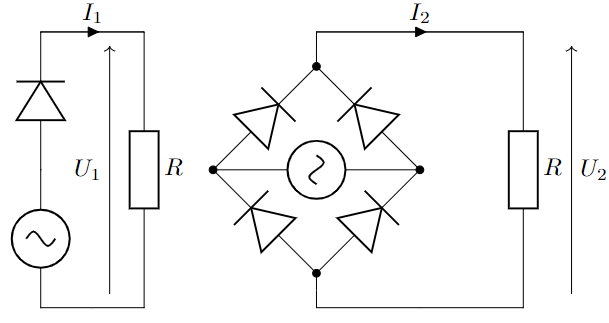
\includegraphics[scale=0.5]{images/4.png}
    \caption{Redresseur de tension}
    \end{center}
\end{figure}

\underline{$\star$ Rappel :}

$V_{eff}=\sqrt{2}*V_{max}$
$V_{max}=\frac{V_{pp}}{4}$
$V_{moy}=\frac{V_{max}}{2\pi}$

Voici l'allure des composants $U_1$, $U_2$, $I_1$ et $I_2$, sachant que $R=1k\Omega$ et $V_{PP}=5V$ :


\begin{figure}[H]
    \begin{center}
    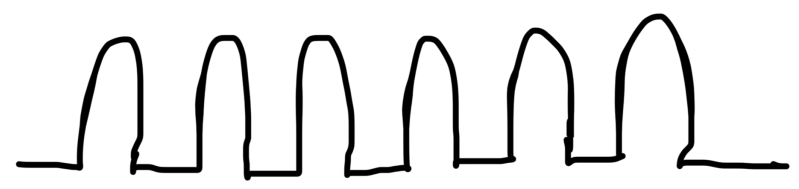
\includegraphics[scale=0.5]{images/boucle1.png}
    \caption{Allure de $U_1$ et $I_1$}
    \end{center}
\end{figure}

\begin{figure}[H]
    \begin{center}
    
\includegraphics[scale=0.5]{images/boucle2.png}
    \caption{Allure de $U_2$ et $I_2$}
    \end{center}
\end{figure}

\newpage
Calculons ensuite les valeurs moyennes et efficaces de $U_1$ et $U_2$ :

\[V{pp}=5V\]
\[V_{moy1}=\frac{V_{max1}}{2\pi} \simeq 0.39V\]
\[V_{eff1}=\frac{V_{max1}}{\sqrt{2}}= 0.884V\]

\[V_{max2}=2V_{moy1}\simeq0.78V\]
\[V_{eff2}=\sqrt{2}*1.25=0.884V\]


La valeur moyenne de $U_1$ est de $0.39V$ et la valeur efficace est de $0.884V$. Pour $U_2$, la valeur moyenne est de $0.78V$ et la valeur efficace est de $0.884V$.

\newpage
\subsection{Redresseur mono-alternance}

Nous avons réalisé le premier circuit et avons mesuré la tension aux bornes de la résistance $R$ appelée $U_1$. Voici l'oscillogramme correspondant :

\begin{figure}[H]
    \begin{center}
    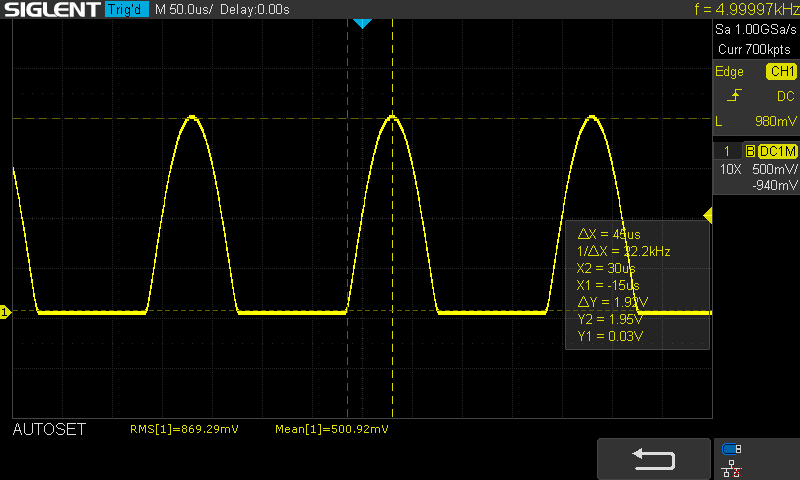
\includegraphics[scale=0.5]{images/Oscillo/SDS00006.png}
    \caption{Oscillogramme de la tension $U_1$ avec $R=1K\Omega$.}
    \end{center}
\end{figure}
Nous pouvons voir sur la capture d'écran précédente que la tension moyenne est de $869.29mV$ et la tension efficace est de $500.92mV$ . Nous avons donc des résultats proches de ceux calculés précédemment.

Ensuite, nous avons ajouté un condensateur de $1\mu F$ en parallèle de la résistance $R$ et avons mesuré la tension aux bornes de ce dernier. Voici l'oscillogramme correspondant :

\begin{figure}[H]
    \begin{center}
    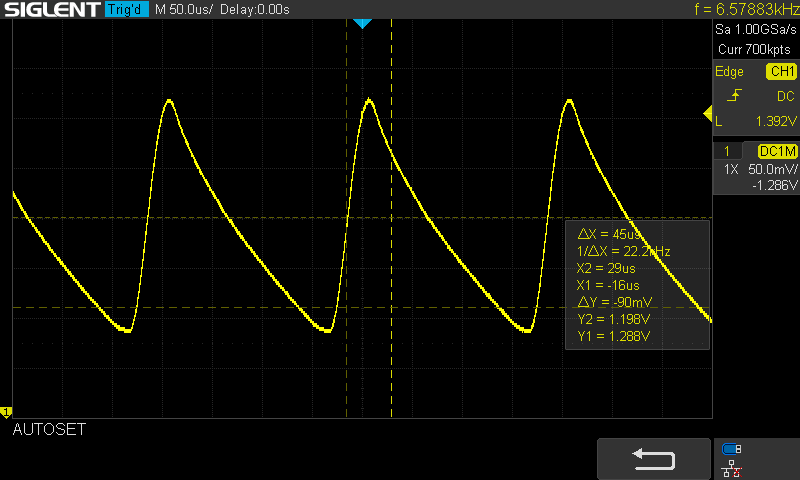
\includegraphics[scale=0.5]{images/Oscillo/SDS00003.png}
    \caption{Oscillogramme de la tension $U_1$ avec $R=1k\Omega$ et $C=1\mu F$.}
    \end{center}
\end{figure}

Nous pouvons déduire de la courbe précédente que des sortes de pics se forment, ce qui est dû au condensateur qui se charge et se décharge.

Après quoi, nous avons modifié la résistance pour une résistance de $10k\Omega$ et avons mesuré la tension aux bornes de la résistance. Voici l'oscillogramme correspondant :
\begin{figure}[H]
    \begin{center}
    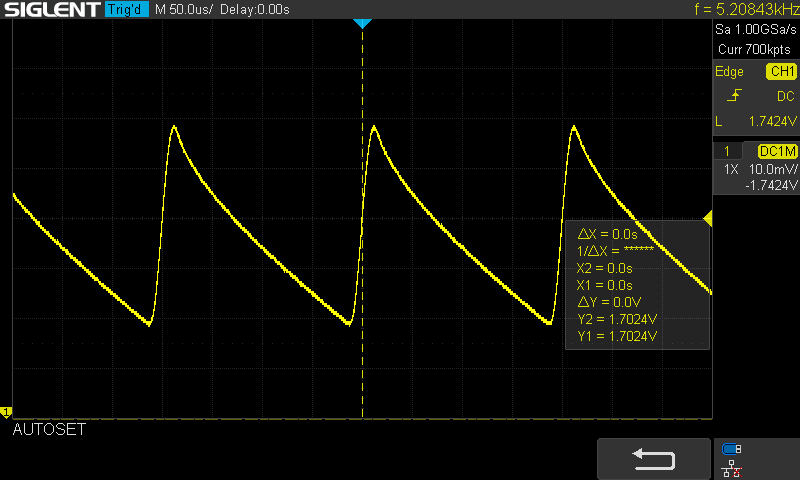
\includegraphics[scale=0.4]{images/Oscillo/SDS00004.png}
    \caption{Oscillogramme de la tension $U_1$ avec $R=10k\Omega$ et $C=1\mu F$.}
    \end{center}
\end{figure}




\newpage
\subsection{Redresseur double-alternance}
\subsubsection{Filtrage simple}

\begin{figure}[H]
    \begin{center}
    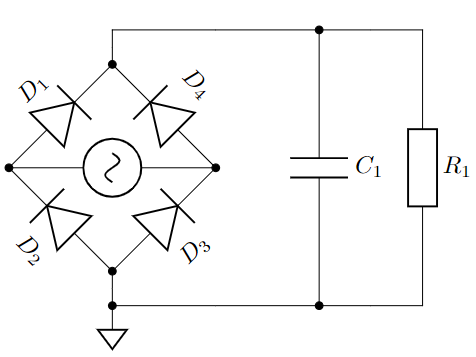
\includegraphics[scale=0.5]{images/5.png}
    \caption{Filtrage simple}
    \end{center}
\end{figure}

Nous avons reproduis le circuit précédent sur LTSPICE, voici son rendu : 

\begin{figure}[H]
    \begin{center}
    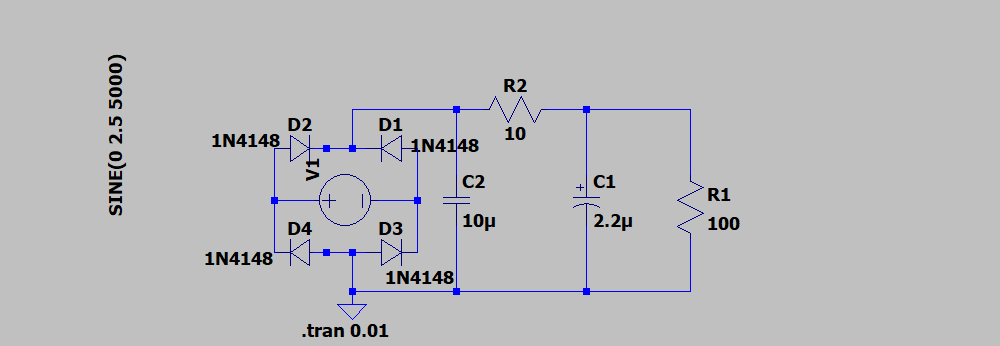
\includegraphics[scale=0.4]{images/LTSPICE/1.png}
    \caption{Filtrage simple sur LTSPICE}
    \end{center}
\end{figure}

Ensuite, nous représenté l’allure de la tension aux bornes de $R_1$ sur $10 ms$ avec différentes valeurs de $R_1$ : $10k\Omega$ ; $5.6k\Omega$ ;
$2.2k\Omega$ ; $1k\Omega$ ; $560\Omega$ ; $220\Omega$ ; $100\Omega$, que voici : 

\begin{figure}[H]
    \begin{center}
    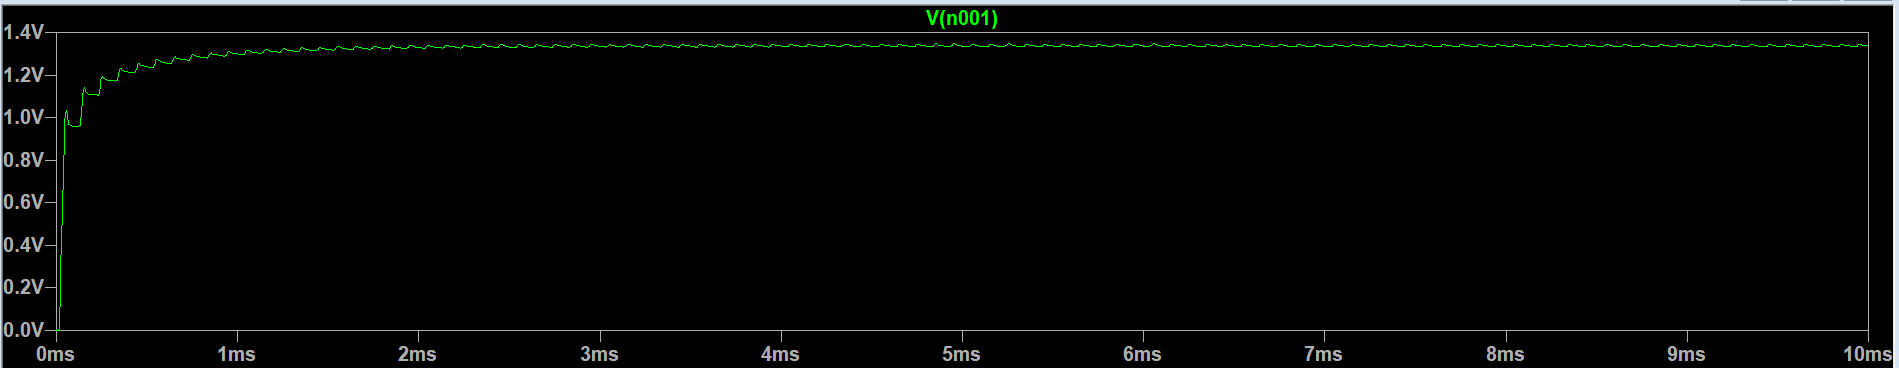
\includegraphics[scale=0.25]{images/LTSPICE/2.png}
    \caption{$R=10k\Omega$}
    \end{center}
\end{figure}

\begin{figure}[H]
    \begin{center}
    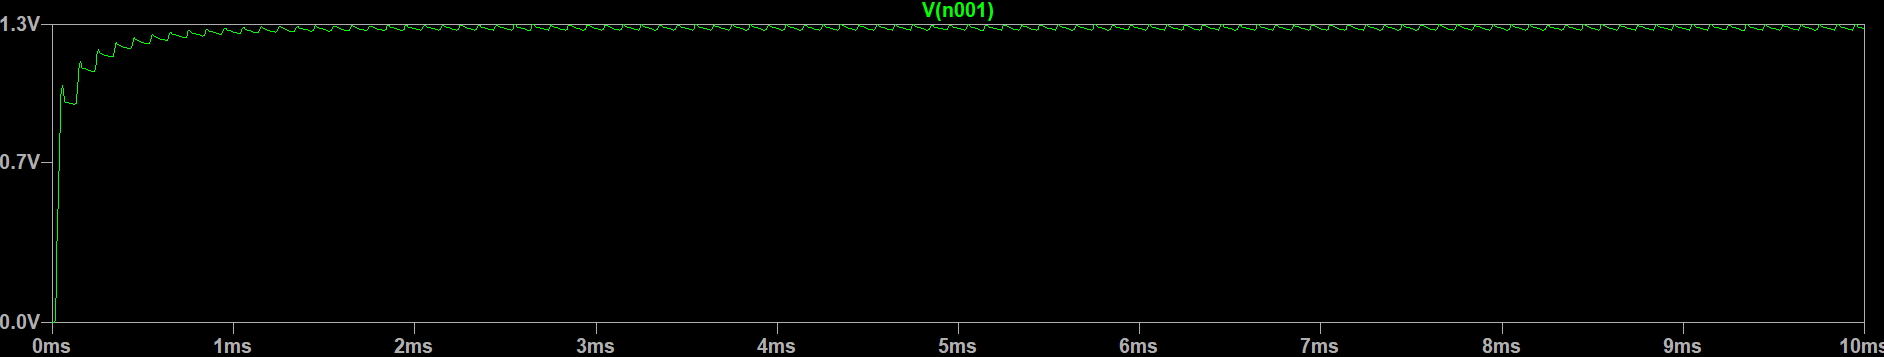
\includegraphics[scale=0.25]{images/LTSPICE/3.png}
    \caption{$R=5.6k\Omega$}
    \end{center}
\end{figure}

\begin{figure}[H]
    \begin{center}
    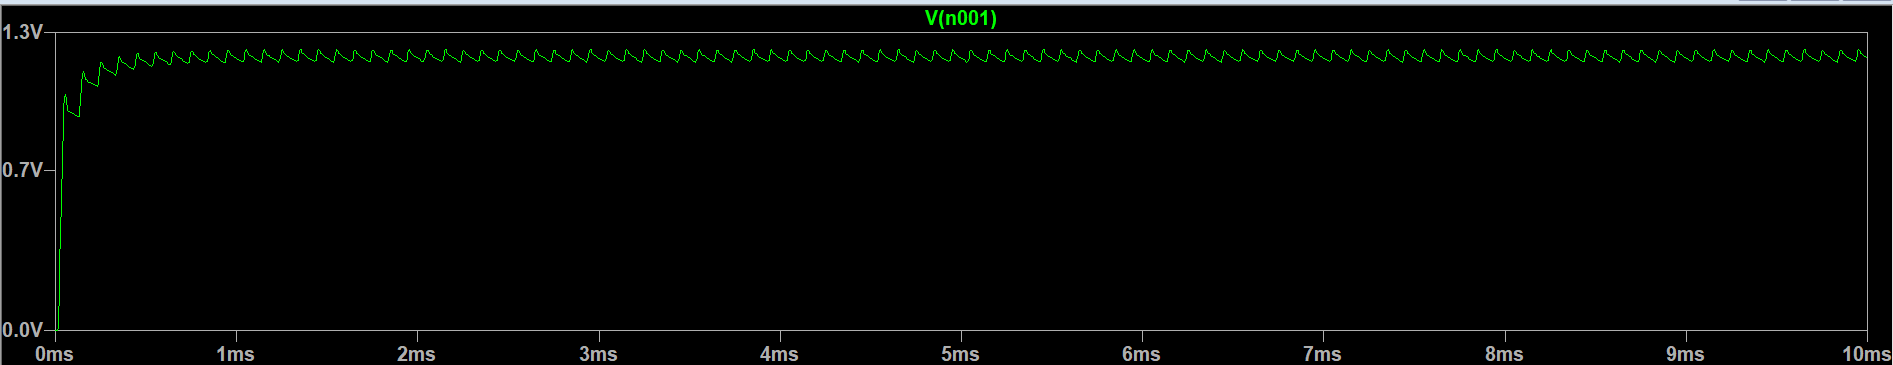
\includegraphics[scale=0.25]{images/LTSPICE/4.png}
    \caption{$R=2.2k\Omega$}
    \end{center}
\end{figure}

\begin{figure}[H]
    \begin{center}
    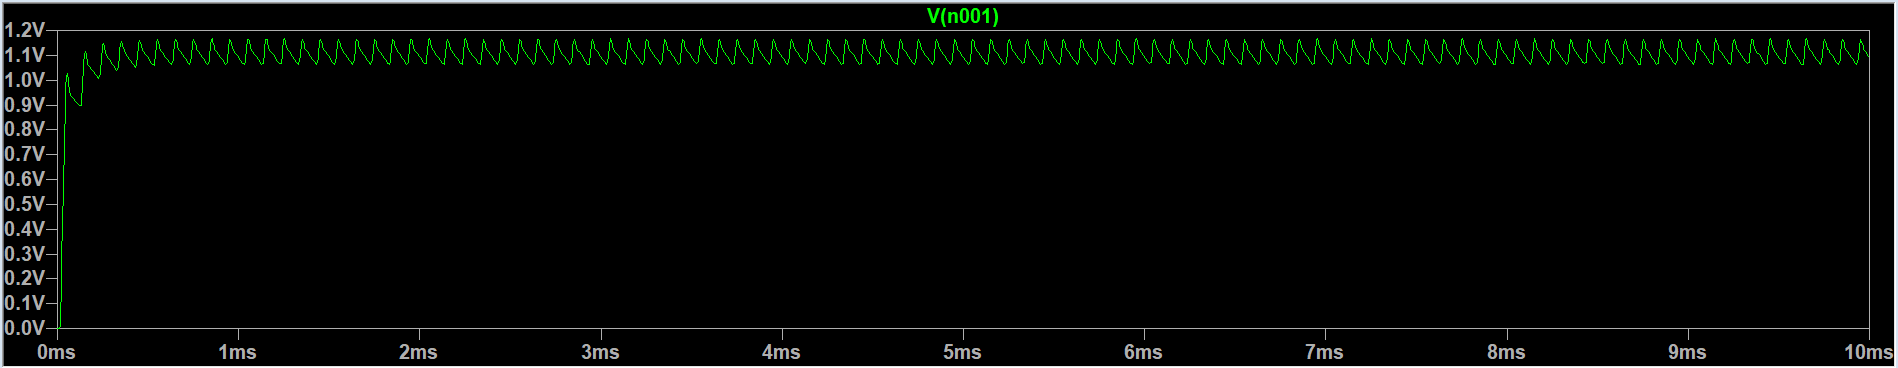
\includegraphics[scale=0.25]{images/LTSPICE/5.png}
    \caption{$R=1k\Omega$}
    \end{center}
\end{figure}

\begin{figure}[H]
    \begin{center}
    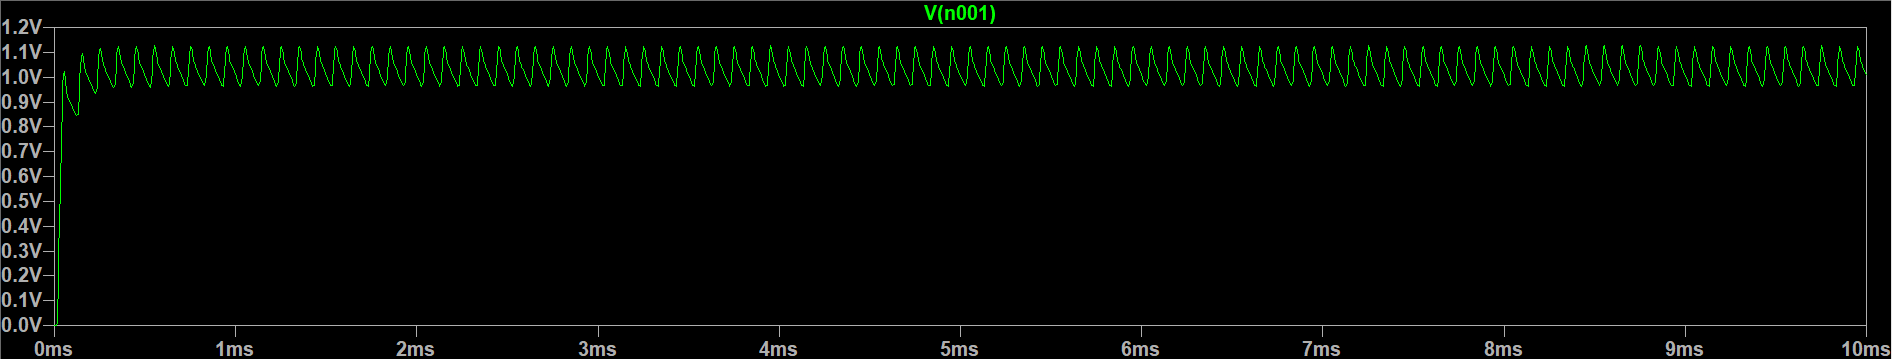
\includegraphics[scale=0.25]{images/LTSPICE/6.png}
    \caption{$R=560\Omega$}
    \end{center}
\end{figure}

\begin{figure}[H]
    \begin{center}
    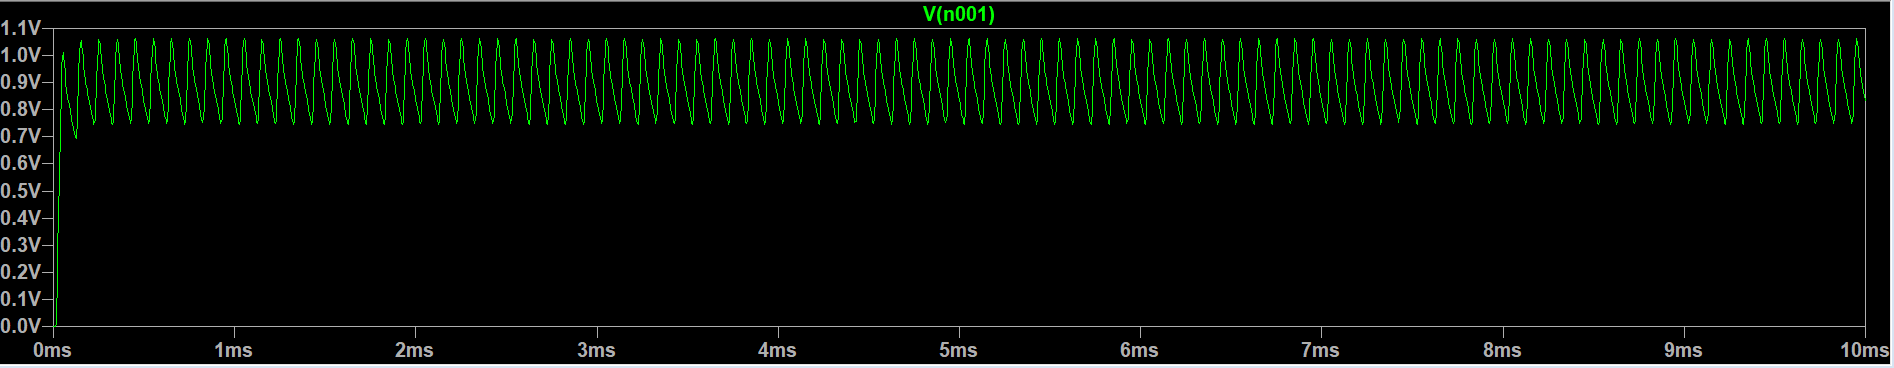
\includegraphics[scale=0.25]{images/LTSPICE/7.png}
    \caption{$R=220\Omega$}
    \end{center}
\end{figure}

\begin{figure}[H]
    \begin{center}
    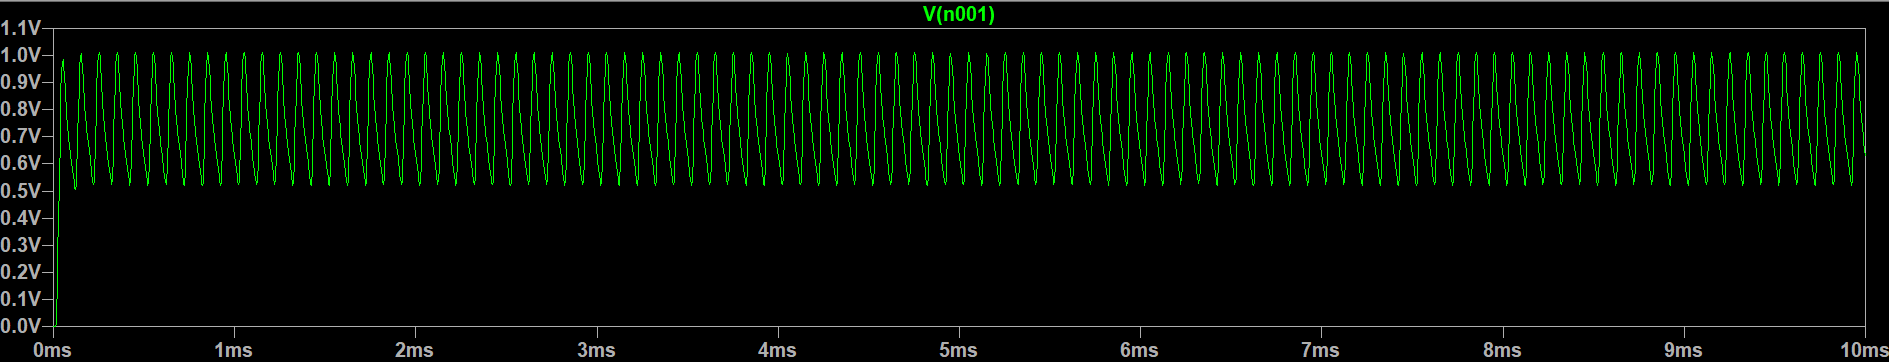
\includegraphics[scale=0.25]{images/LTSPICE/8.png}
    \caption{$R=100\Omega$}
    \end{center}
\end{figure}

Nous pouvons en conclure que lorsque $R_1$ diminue, le signal oscille de plus en plus et la tension maximale diminue.


\subsubsection{Filtrage double}

\begin{figure}[H]
    \begin{center}
    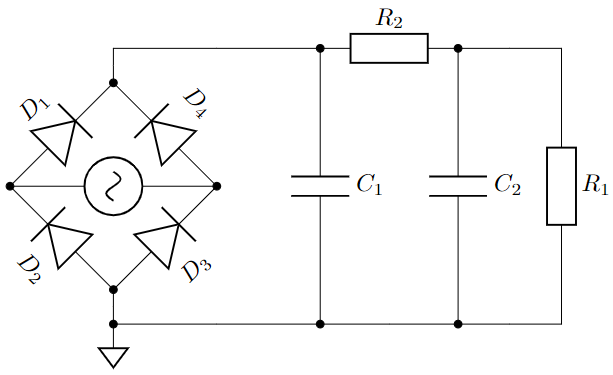
\includegraphics[scale=0.5]{images/6.png}
    \caption{Filtrage double}
    \end{center}
\end{figure}

Nous avons reproduis le circuit précédent sur LTSPICE, voici son rendu :

\begin{figure}[H]
    \begin{center}
    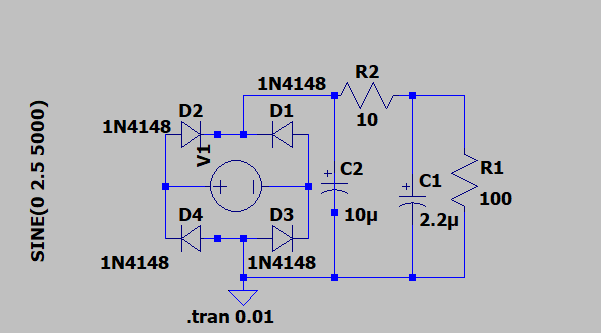
\includegraphics[scale=0.4]{images/LTSPICE/a.png}
    \caption{Filtrage double sur LTSPICE}
    \end{center}
\end{figure}

Ensuite, nous représenté l’allure de la tension aux bornes de $R_1$ sur $10 ms$ avec différentes valeurs de $R_1$ : $10k\Omega$ ; $5.6k\Omega$ ; $2.2k\Omega$ ; $1k\Omega$ ; $560\Omega$ ; $220\Omega$ ; $100\Omega$, que voici : 

\begin{figure}[H]
    \begin{center}
    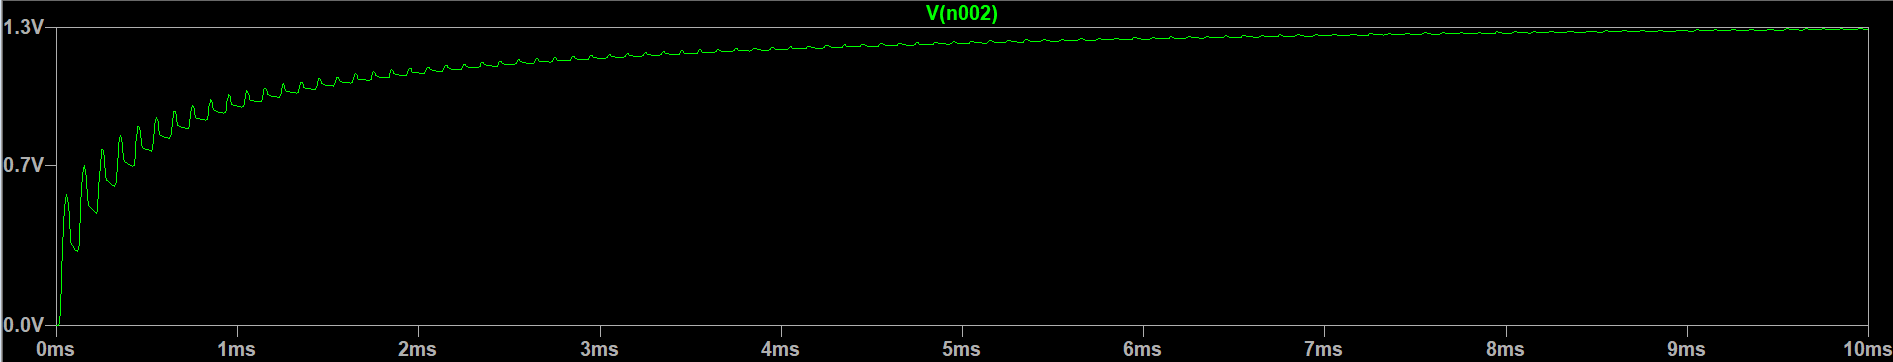
\includegraphics[scale=0.25]{images/LTSPICE/b.png}
    \caption{$R=10k\Omega$}
    \end{center}
\end{figure}

\begin{figure}[H]
    \begin{center}
    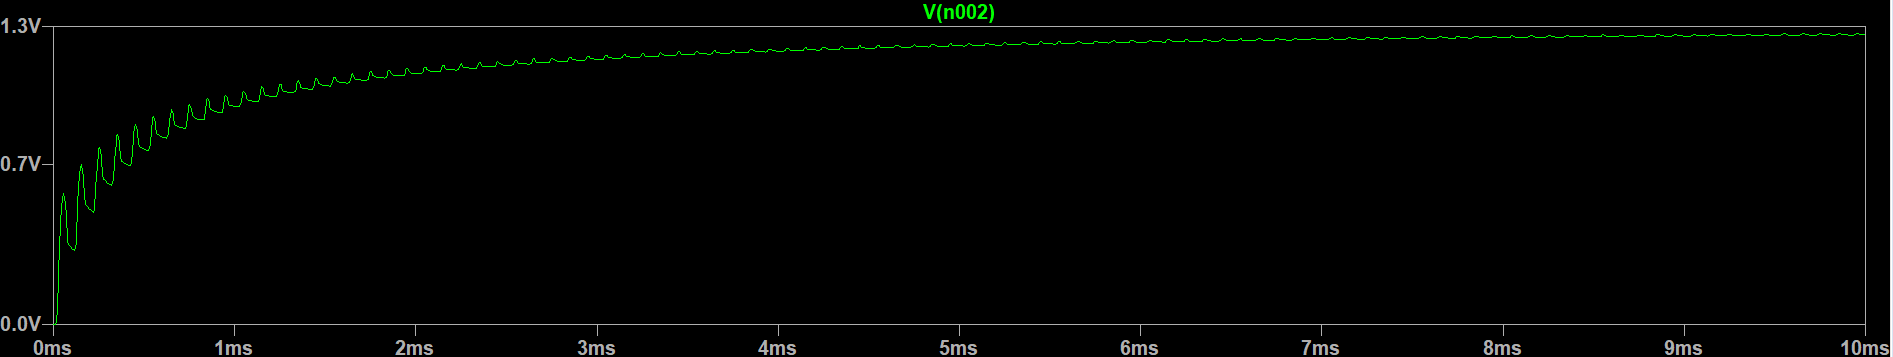
\includegraphics[scale=0.25]{images/LTSPICE/c.png}
    \caption{$R=5.6k\Omega$}
    \end{center}
\end{figure}

\begin{figure}[H]
    \begin{center}
    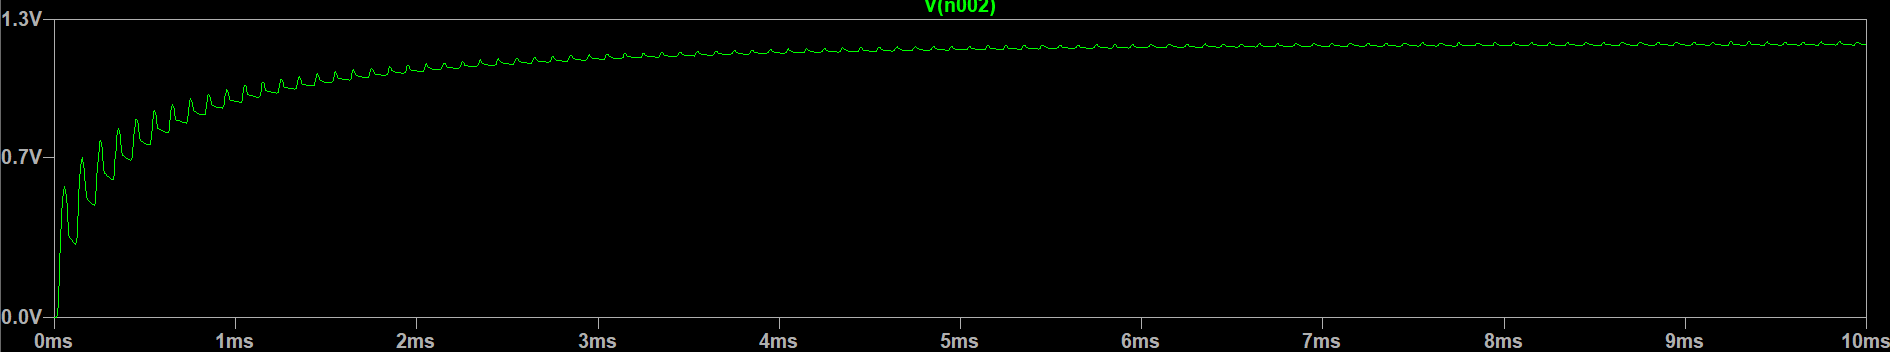
\includegraphics[scale=0.25]{images/LTSPICE/d.png}
    \caption{$R=2.2k\Omega$}
    \end{center}
\end{figure}

\begin{figure}[H]
    \begin{center}
    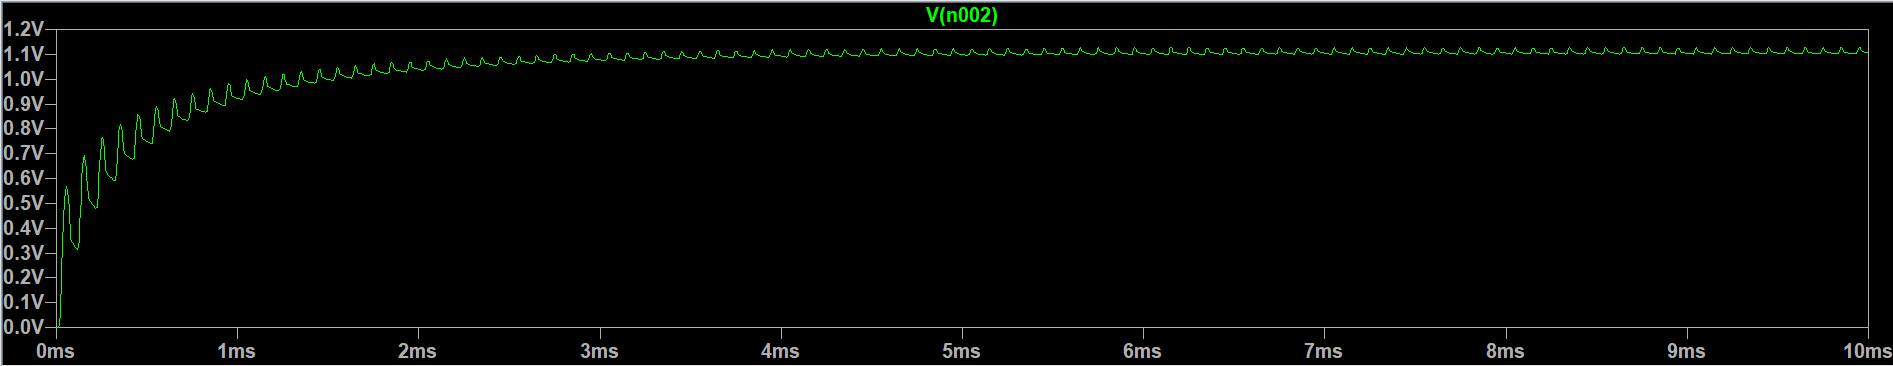
\includegraphics[scale=0.25]{images/LTSPICE/e.png}
    \caption{$R=1k\Omega$}
    \end{center}
\end{figure}

\begin{figure}[H]
    \begin{center}
    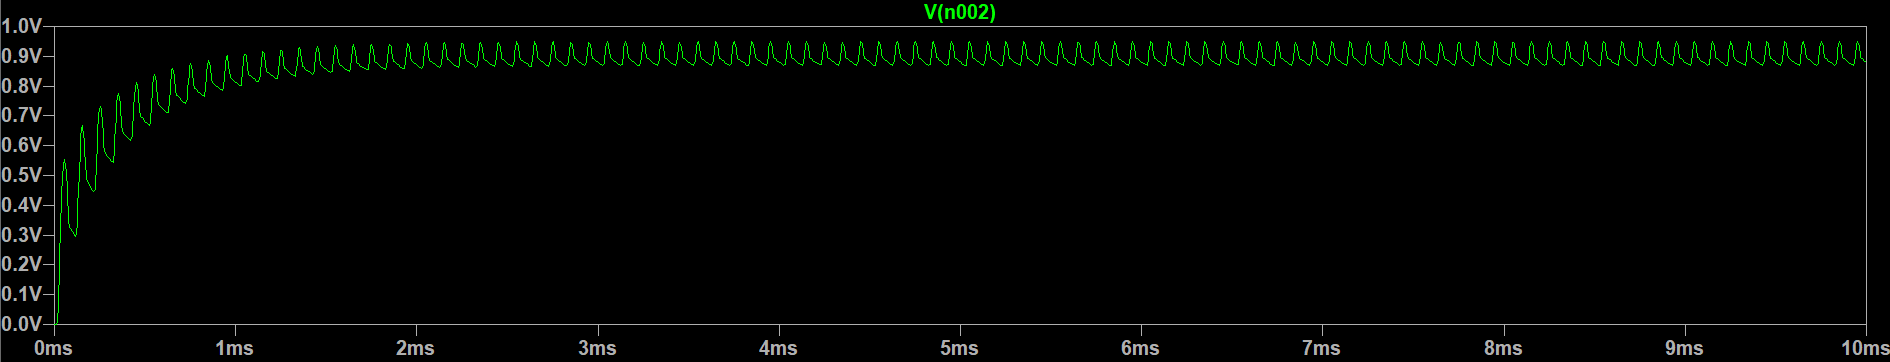
\includegraphics[scale=0.25]{images/LTSPICE/f.png}
    \caption{$R=560\Omega$}
    \end{center}
\end{figure}

\begin{figure}[H]
    \begin{center}
    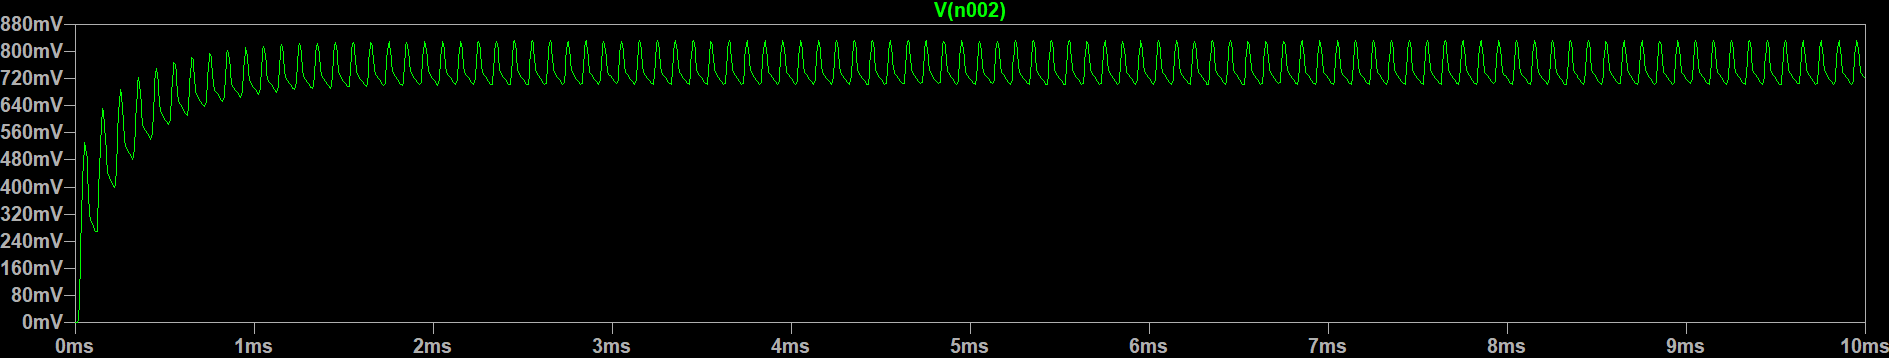
\includegraphics[scale=0.25]{images/LTSPICE/g.png}
    \caption{$R=220\Omega$}
    \end{center}
\end{figure}

Nous pouvons voir que le signal est meilleur qu'avant : cela est dû au fait que le filtrage double est plus efficace que le filtrage simple, avec les deux condensateurs en parallèle.
\\
Cependant, le principal inconveniant de ce montage est que le signal est déphasé de $\frac{\pi}{2}$, ce qui peut poser problème dans certaines applications. De plus, il est nécessaire d'avoir un composants suplémentaire.

\newpage
\section{Conclusion} 
Pour conclure ce TP final, nous avons réutilisé différentes notions vues dans les TP précédents en les appliquant avec les diodes. Le côté pratique avec les différents montage réalisés, ainsi que l’utilisation à nouveau de LTSpice. Encore une fois, côté LaTex, nous avons pu nous améliorer pour tracer des courbes et pour mieux structurer notre rapport.
\\
Enfin, je pense que cette deuxième année de TP nous a permis d'avoir une meilleure démarche scientifique lors d'expériences et sommes désormais prêts pour des réalisations plus complexes.

}
\end{document}